\section{系统测试报告}
\begin{frame}{测试用例设计}
    黑盒测试,主要采用场景法设计用例,大约设计了60个左右的Testcases:
    \begin{table}[]
        \centering
        \resizebox{\textwidth}{!}{
            \begin{tabular}{c|c|c|c}
                \textbf{功能点/issue}       & \textbf{测试用例id} & \textbf{测试用例}                                                & \textbf{优先级} \\
                \hline
                账号管理-用户注册           & TC001               & 正常注册流程,在注册界面中输入相关信息,点击注册,显示注册成功   & 最高            \\
                \hline
                账号管理-用户注册           & TC002               & 在注册时用户账号已被注册,提示失败并且结束用例                   & 高              \\
                \hline
                账号管理-用户注册           & TC003               & 在注册时邮箱已经被绑定,提示失败并且结束用例                     & 高              \\
                \hline
                账号管理-用户注册           & TC004               & 在注册时未将表单填写完整,提示无法提交注册表单并显示未填写的字段 & 高              \\
                \hline
                账号管理-用户登录           & TC005               & 正常登录流程,输入账号密码后成功 登录                            & 最高            \\
                \hline
                账号管理-用户登录           & TC006               & 登录时账号不存在,提示登录失败                                   & 高              \\
                \hline
                账号管理-用户登录           & TC007               & 登录时账号密码错误,提示登录失败                                 & 高              \\
                \hline
                项目管理-项目搜索           & TC008               & 正常搜索流程,输入搜索内容输出匹配项目                           & 最高            \\
                \hline
                项目管理-项目新建           & TC009               & 正常创建流程,点击新建项目输入项目信息后创建                     & 最高            \\
                \hline
                项目管理-查看项目上传的文件 & TC010               & 用户查看不存在的项目文件                                         & 中              \\
                \hline
                项目管理-查看所有项目       & TC011               & 正常查看所有项目                                                 & 最高            \\
                \hline
                项目管理-重命名             & TC012               & 正常重命名项目                                                   & 最高            \\
                \hline
                项目管理-重命名             & TC013               & 用户输入空项目名字后点击确认,应当提示失败                       & 中              \\
                \hline
                项目管理-上传封面           & TC014               & 正常上传项目封面                                                 & 最高            \\
                \hline
                项目管理-上传封面           & TC015               & 上传非图片格式的封面文件                                         & 中              \\
                \hline
                项目管理-删除项目           & TC016               & 正常删除项目                                                     & 最高            \\
                \hline
                项目管理-项目新建           & TC017               & 新建具有相同名字的项目                                           & 中              \\
                \hline
                项目管理-上传文件           & TC018               & 正常上传文件                                                     & 最高            \\
                \hline
                项目管理-上传文件           & TC019               & 上传大小大于100MB的大文件                                        & 中              \\
                \hline
                项目管理-上传文件           & TC020               & 编辑上传文件的文件名                                             & 最高            \\
            \end{tabular}
        }
        \caption{部分测试用例展示}
        \label{tab:tech-strategy}
    \end{table}
\end{frame}

\begin{frame}{需求覆盖分析}
    \begin{table}[]
        \centering
        \resizebox{\textwidth}{!}{
            \begin{tabular}{c|c|c}
                \textbf{测试用例id} & \textbf{是否通过} & \textbf{备注}                                                                                     \\
                \hline
                TC001               & 通过              & 无                                                                                                \\
                \hline
                TC002               & 通过              & 无                                                                                                \\
                \hline
                TC002               & 通过              & 无                                                                                                \\
                \hline
                TC003               & 不通过            & 只实现了登录时填写邮箱信息,未实现验证功能                                                        \\
                \hline
                TC004               & 通过              & 无                                                                                                \\
                \hline
                TC005               & 通过              & 无                                                                                                \\
                \hline
                TC006               & 通过              & 无                                                                                                \\
                \hline
                TC007               & 通过              & 无                                                                                                \\
                \hline
                TC008               & 通过              & 但搜索不存在的项目时,界面不太友好,未出现相应提示信息,界面不变;界面的时间显示紊乱              \\
                \hline
                TC009               & 通过              & 无                                                                                                \\
                \hline
                TC010               & 通过              & 无                                                                                                \\
                \hline
                TC011               & 通过              & 无                                                                                                \\
                \hline
                TC012               & 通过              & 无                                                                                                \\
                \hline
                TC013               & 不通过            & 能重命名项目为空;能创建多个名字相同的项目;重命名后后缀丢失,PPT文件重命名(未加后缀)后无法打开 \\
                \hline
                TC014               & 通过              & 无                                                                                                \\
                \hline
                TC015               & 不通过            & 无                                                                                                \\
                \hline
                TC016               & 通过              & 无                                                                                                \\
                \hline
                TC017               & 不通过            & 无                                                                                                \\
                \hline
                TC018               & 通过              & 无                                                                                                \\
                \hline
                TC019               & 不通过            & 文件过大时无法上传                                                                                \\
                \hline
                TC020               & 不通过            & 修改上传文件名时网页总是提示错误信息                                                              \\
                \hline
            \end{tabular}
        }
        \caption{部分需求覆盖展示}
        \label{tab:tech-strategy}
    \end{table}
\end{frame}

\begin{frame}{缺陷统计}
    \begin{table}[]
        \centering
        \resizebox{\textwidth}{!}{
            \begin{tabular}{c|c|c|c|c|c|c}
                \textbf{序号} & \textbf{Bug描述}                                                                       & \textbf{重要性等级} & \textbf{所属模块} & \textbf{是否修复}     & \textbf{尚未修复}                & \textbf{备注}                                                                \\
                \hline
                1             & 项目中的非PPT的json文件后出现打开按钮(正常应该只出现在PPT文件后),点击后卡在加载页面 & 一般                & 项目管理          & 是                    &                                  &                                                                    \\
                \hline
                2             & 用户可以操作非自己创建的项目,如删除、重命名文件                                       & 一般                & 项目管理          & 是                    &                                  &                                                                    \\
                \hline
                3             & 注册时有要求填写邮箱信息,但在注册界面并没有实现验证功能                               & 一般                & 账号管理          & 是                    &                                  &                                                                    \\
                \hline
                4             & 项目可以重命名为空                                                                     & 较严重              & 项目管理          & 是                    &                                  &                                                                    \\
                \hline
                5             & 项目可以重名                                                                           & 一般                & 项目管理          & \multicolumn{1}{r|}{} & \multicolumn{1}{p{4.055em}|}{是} & \multicolumn{1}{p{4.055em}|}{不影响使用,可以准确区分项目的创建者} \\
                \hline
                6             & PPT重命名不加后缀,之后不能打开                                                        & 较严重              & 项目管理          & 是                    &                                  &                                                                    \\
                \hline
                7             & 搜索结果界面的时间显示紊乱                                                             & 一般                & 项目管理          & 是                    &                                  &                                                                    \\
                \hline
                8             & 上传头像/PPT封面时未对文件进行限制                                                     & 较严重              & 项目管理/个人信息 & 是                    &                                  &                                                                    \\
                \hline
                9             & 个人信息修改界面的邮箱验证无效                                                         & 一般                & 个人信息          & 是                    &                                  &                                                                    \\
                \hline
                10            & 搜索界面时间显示紊乱                                                                   & 一般                & 项目管理          & 是                    &                                  &                                                                    \\
                \hline
            \end{tabular}
        }
        \caption{部分缺陷统计展示}
        \label{tab:tech-strategy}
    \end{table}
\end{frame}

\begin{frame}{性能测试}
    \begin{itemize}
    \item 性能测试中,我们主要使用Apifox测试了软件系统同时并发支持用户注册登录的性能表现,发现随着并发用户数量的增加,服务器的响应时间和吞吐量也相应增加,但在达到某个阈值后,这两个指标开始稳定。这意味着软件系统能够在一定的并发访问量下保持高效的处理能力。
    \item 当并发用户数量进一步增加,服务器的错误率也开始增加。这表明在极端的并发访问情况下,系统可能会遇到性能瓶颈,这是可能需要进一步优化的地方。
    \end{itemize}
\end{frame}

\begin{frame}{性能测试}
    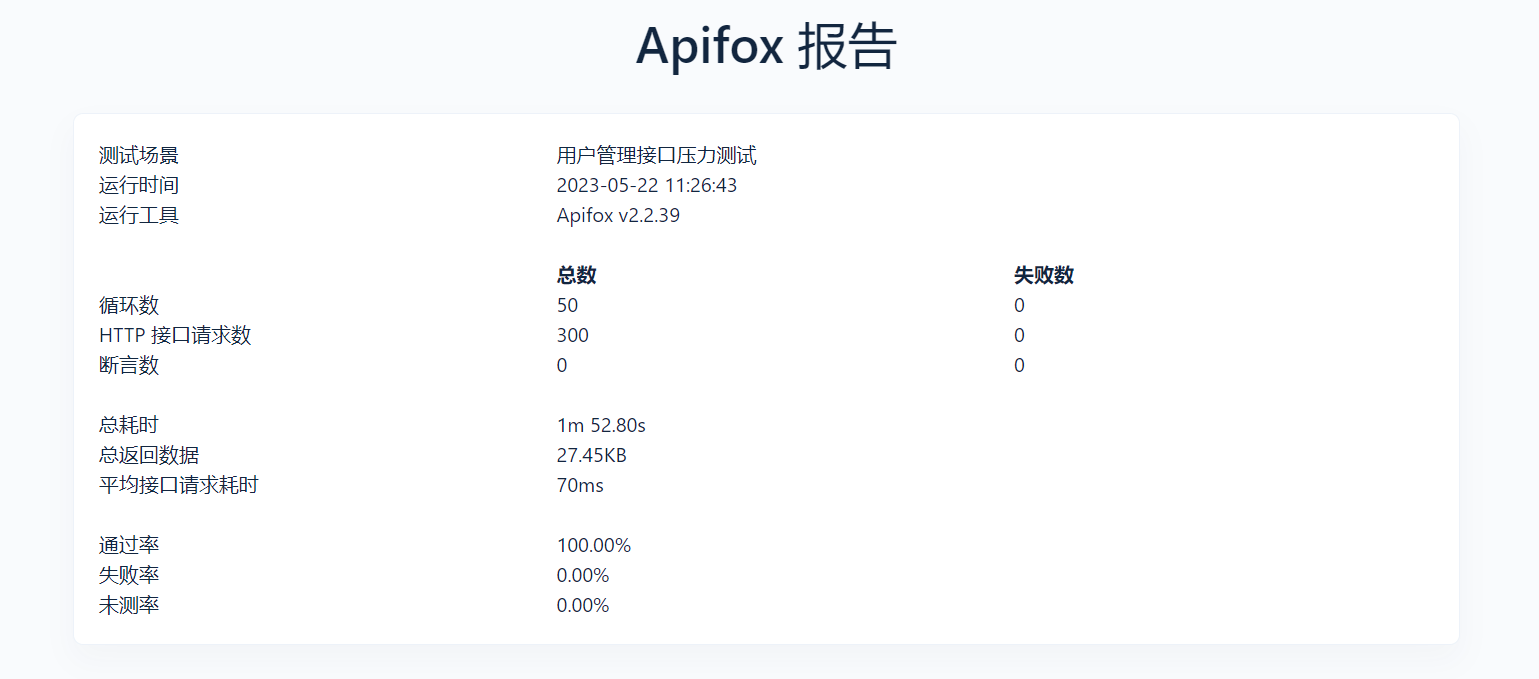
\includegraphics[width=\textwidth]{contents/figure/apifox_report.png}
\end{frame}

